%&latex
\documentclass{article}

\usepackage{tikz}
\usetikzlibrary{automata,arrows}

\begin{document}
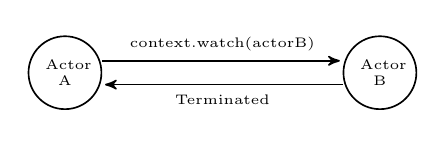
\begin{tikzpicture}[->,>=stealth',shorten >=1pt,auto,node distance=4cm,semithick,font=\tiny]
  \tikzstyle{every state}=[fill=none,draw=black,text=black, text centered, text width=0.5cm]

  \node[state] (A) {Actor A};
  \node[state] (B) [right of=A] {Actor B};

  \path ([yshift=1ex]A.east) edge node {context.watch(actorB)} ([yshift=1ex]B.west);
  \path ([yshift=-1ex]B.west) edge node {Terminated} ([yshift=-1ex]A.east);

\end{tikzpicture}

\end{document}
